\documentclass{article}
\usepackage{amsmath, amssymb, tikz, geometry, graphicx, natbib, mwe, color, xcolor, listings, tabularx, pdfpages, blindtext, mathtools, stackengine, pgfplots,bigints, relsize, upgreek, esint, array, multirow, schemata, wrapfig, cancel, comment}
\usepackage{hyperref}
\usepackage{slashed, enumitem}
\usepackage{titlesec}
\usetikzlibrary{positioning}

\begin{comment}
code to write section, subsection and subsubsection title in a specific color
\titleformat{\section}
{\color{synthwave_text}\normalfont\Large\bfseries}
{\color{synthwave_text}\thesection}{1em}{} 

\titleformat{\subsection}
{\color{synthwave_text}\normalfont\large\bfseries}
{\color{synthwave_text}\thesubsection}{1em}{} 

\titleformat{\subsubsection}
{\color{synthwave_text}\normalfont\normalfont\bfseries}
{\color{synthwave_text}\thesubsubsection}{1em}{}
\end{comment}


\pgfplotsset{compat=1.9}

\colorlet{myWhite}{white!35!gray}
\definecolor{shadeofgray}{HTML}{181818}
\definecolor{shadeofviolet}{HTML}{0f022c}
\definecolor{synthwave_beckground}{HTML}{252334}
\definecolor{synthwave_text}{HTML}{e148aa}


\hypersetup{
    colorlinks=true,
    linkcolor=violet,
    filecolor=magenta,      
    urlcolor=cyan,
    pdftitle={Tecnologie Web T},
    pdfpagemode=FullScreen,
}


\geometry{ 
 a4paper,
 left=10mm,
 right=10mm,
 top=10mm
 }
 
\lstdefinestyle{mystyle}{ 
bracketsstyle=\color{red}
}

\title{Tecnologie Web T}
\author{Giuseppe Bumma}


% color option
%\pagecolor{synthwave_beckground} %{shadeofgray}
%\color{myWhite}

\renewcommand{\CancelColor}{\color{synthwave_text}}


\begin{document}

%Commands
\newcommand{\R}{\mathbb{R}}
\newcommand{\Varepsilon}{\mathcal{E}}
\newcommand{\rad}{\text{rad}}
\newcommand{\bb}[1]{\mathbb{#1}}
\newcommand{\cc}[1]{\mathcal{#1}}
\newcommand{ \lognormal }{\text{Lognormal} }
\newcommand{\T}[1]{\text{#1}}
\newcommand*\circled[1]{\tikz[baseline=(char.base)]{%
            \node[shape=circle,draw,inner sep=2pt] (char) {#1};}}
%for using circled number in enumerate use:
%\begin{enumerate}[label=\protect\circled{\arabic*}]


\tableofcontents

\maketitle

\section{Introduzione}
Il World Wide Web (WWW) è stato proposto nel 1989 da Tim
Berners-Lee, ricercatore di fisica al CERN di Ginevra.\\
L'idea alla base del progetto era quella di fornire
strumenti adatti a condividere:
\begin{itemize}
    \item documenti statici
    \item in forma ipertestuale
    \item disponibili su rete Internet tramite protocollo
    semplice e leggero
\end{itemize}
Si volevano rimpiazzare i sistemi di condivisione di documenti basati su protocolli più vecchi come FTP e Gopher.
\subsection{Storia}
\begin{itemize}
    \item Nel marzo del 1989 Tim Berners-Lee
    elaborò una proposta
    \item Il 12 novembre 1990 assieme a Robert
    Cailliau presentò una proposta più
    formale per un sistema ipertestuale
    basato su un'architettura client-server
    \item Il 6 agosto 1991 Berners-Lee mise
    on-line su Internet il primo sito Web
    Inizialmente fu utilizzato solo dalla
    comunità scientifica
    \item Il 30 aprile 1993 il CERN decise di
    rendere pubblica la tecnologia alla
    base del Web
\end{itemize}
L'HTTP (\textbf{HyperText Transfer Protocol}) è un protocollo che sta alla base dell'internet e che permette lo scambio di informazioni in architetture client-server. Ci sono state varie implementazioni del protocollo HTTP
\begin{itemize}
    \item HTTP/1.0, implementato nel 1991 e
    proposto come Request for Comment
    RFC 1945 a Internet Engineering Task
    Force IETF nel 1996
    \item HTTP/1.1, presentato come RFC
    2068 nel 1997 e aggiornato/approvato
    nel 1999 come RFC 2616
    \item HTTP/2 (origin. chiamato HTTP/2.0),
    basato su SPDY, sviluppato dal Working
    Group Hypertext Transfer Protocol
    (httpbis) di IETF
    \item HTTP/2 pubblicato come RFC 7540 a Maggio 2015, 63\% circa del traffico secondo le ultime statistiche
\end{itemize}



\subsection{Gli ipertesti}
Un \textbf{ipertesto} (hypertext) è un insieme di documenti messi in relazione tra loro tramite collegamenti monodirezionali (hyperlink o più semplicemente link). Può essere visto come una rete (un
grafo) e i documenti ne costituiscono i nodi.
\begin{center}
    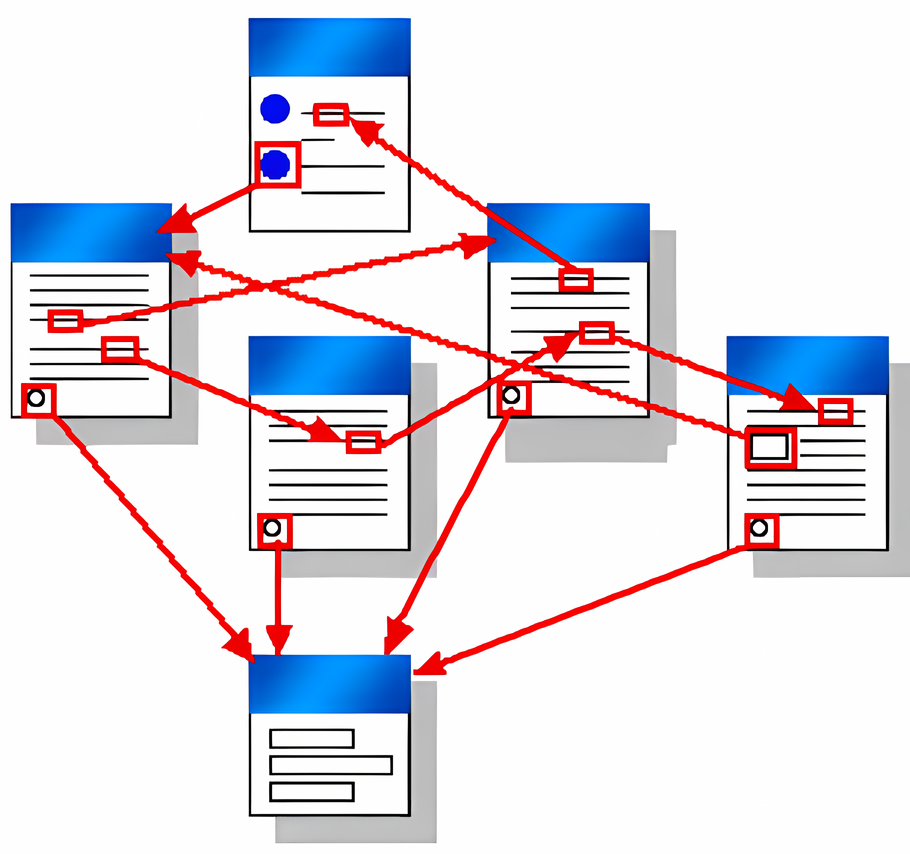
\includegraphics[scale=0.17]{Images/Ipertesto.png}
\end{center}
Attraverso un link possiamo passare da un
punto di un documento ad un altro qualunque dei documenti del grafo. La caratteristica principale di un ipertesto è che la lettura può svolgersi in maniera non lineare: qualsiasi documento della rete può essere il successivo.\\
Se si prendono in considerazione non solo testi ma elementi multimediali (immagini suoni, video) si parla di ipermedia.


\subsection{WWW come sistema ipertestuale}
Idea (e motivazione di successo) di Berners-Lee è stata quella di mettere insieme le idee di ipertesto e rete Internet in modo efficace. World Wide Web è in pratica un ipertesto distribuito sulla rete in cui i documenti, chiamati anche pagine, risiedono su server geograficamente distribuiti (World Wide) e costituiscono una ragnatela virtuale (Web). Da un qualunque documento è possibile “saltare” ad un altro indipendentemente da dove questo si trovi.
\vspace*{0.2cm}\\
Per realizzare questo ipertesto planetario abbiamo
bisogno di tre elementi concettuali:
\begin{itemize}
    \item un meccanismo per localizzare un documento     
    \item un protocollo per accedere alle risorse che costituiscono il documento e trasferirle al client
    \item un linguaggio per descrivere i documenti ipertestuali (usato per costruire le pagine)
\end{itemize}
e di due elementi fisici:
\begin{itemize}
    \item un server in grado di erogare le risorse che costituiscono i documenti
    \item Un client in grado di rappresentare/visualizzare i documenti e di consentire la navigazione da un documento all'altro
\end{itemize}













\end{document}